\documentclass[12pt, letterpaper]{article}
\usepackage{graphicx}
\usepackage[margin=1in]{geometry}
\usepackage{amsmath, amssymb, amsthm, mathrsfs}
\usepackage{fancyhdr}
\usepackage{tikz}
\usepackage{enumerate}
\usepackage{cancel}
\usetikzlibrary{positioning}
\usepackage[utf8]{inputenc}
\usepackage{xcolor}
\usepackage{framed}
\newlength{\hwprobnumwd}
\settowidth{\hwprobnumwd}{\textbf{99.}}
\newcommand{\problemnum}[1]{\makebox[\hwprobnumwd][r]{\textbf{#1.}}}
\title{HW 1.3}
\author{Your Name}
\date{\today}
\pagestyle{fancy}
\renewcommand{\headrulewidth}{0pt}
\renewcommand{\footrulewidth}{0pt}
\fancyhf{}
\rhead{
    Zack Abdirashid\\
    3/31/26 \\
    MATH 405
}
\rfoot{Page \thepage}
\begin{document}
\noindent\textbf{\underline{3.1}}\par
\vspace{0.75\baselineskip}
\noindent
\problemnum{10}\begin{tabular}[t]{l}
     What is the maximum number of vertices (internal and leaves) in an $m$-ary tree \\
     of height $h$?
\end{tabular} \\
\indent \indent \begin{tabular}[t]{l}
    \text{Recall by Theorem 3,} $n = mi + l$. We know by Therorem 4, $l \leq m^h$. 
    So, the maximum \# \\ of leaves is $m^h$. By the Corollary in 3.1, $i = \frac{l - 1}{m - 1}$. So,
    \end{tabular}
    \begin{align*}
        n &= mi + l \\
        &= \boxed{m\left(\frac{m^h - 1}{m - 1}\right) + m^h}
    \end{align*}
\noindent
\problemnum{16}\begin{tabular}[t]{l}
    \text{A \textit{forest} is an unconnected graph that is a disjoint union of trees.
    If $G$ is an $n$-vertex forest of} \\
    \text{$t$ trees, how many edges does it have?}
    \end{tabular} \\ 
    \indent \indent \begin{tabular}[t]{l}
        For any tree, it has $n-1$ edges where $n$ is the \# of vertices in the tree. 
        Since there are $t$ trees \\
        in $G$, trees $1$ will have $n_1 - 1$ edges, $2$ with $n_2 - 1$ edges, and $t$ with $n_t - 1$ edges where each \\
        $n_i$ adds up to $n$. So, the \# of edges in $G$ should be
    \end{tabular}  
    \begin{align*}
       &\Rightarrow \ (n_1 - 1) + (n_2 - 1) + \ldots + (n_t - 1) \\
       &\Rightarrow \ \underbrace{(n_1 + n_2 + \ldots + n_t)}_n - \underbrace{(1 + 1 + \ldots + 1)}_{\text{$t$ times}} \\
       &\Rightarrow \ \boxed{n - t}
    \end{align*}
    \hspace{0.5em}  
\problemnum{31} \begin{tabular} [t]{l}
    In the proof of Thereom 5, we showed that a Prufer sequence $(s_{1}, s_{2}, \ldots, s_{n-2})$ uniquely described \\
    a tree on $n$ items. Construct the trees with the following Prufer sequences.
\end{tabular}
\indent $\textbf{(a)} \ (4, 5, 6, 2)$\par
\vspace{0.5\baselineskip}
\begin{center}
\begin{tabular}{@{}c@{\hspace{2.5em}}l@{}}
\begin{tikzpicture}[baseline=(current bounding box.center), scale=1.15]
  \def\rvert{2.1}
  \def\rlabel{2.5}
  \foreach \i [evaluate=\i as \ang using 90-(\i-1)*60] in {1,...,6} {
    \coordinate (v\i) at ({\ang}:\rvert);
    \fill (v\i) circle (2pt);
    \node[inner sep=1pt] at ({\ang}:\rlabel) {\i};
  }
  \draw (v1) -- (v4);
  \draw (v4) -- (v6);

  \draw (v2) -- (v5);
  \draw (v2) -- (v6);

  \draw (v3) -- (v5);
\end{tikzpicture}
&
$V = \{\cancel{1}, \underline{2}, \cancel{3}, \cancel{4}, \cancel{5}, \underline{6}\}$
\end{tabular}
\end{center} \hspace{0.5em}
 \ $\textbf{(b)} \ (2, 8, 8, 3, 5, 4)$\par
\vspace{0.5\baselineskip}
\begin{center}
\begin{tabular}{@{}c@{\hspace{2.5em}}l@{}}
\begin{tikzpicture}[baseline=(current bounding box.center), scale=1.15]
  \def\rvert{2.1}
  \def\rlabel{2.5}
  \foreach \i [evaluate=\i as \ang using 90-(\i-1)*45] in {1,...,8} {
    \coordinate (vb\i) at ({\ang}:\rvert);
    \fill (vb\i) circle (2pt);
    \node[inner sep=1pt] at ({\ang}:\rlabel) {\i};
  }
  \draw (vb1) -- (vb2);
  \draw (vb2) -- (vb8);
  \draw (vb6) -- (vb8);
  \draw (vb7) -- (vb3);
  \draw (vb3) -- (vb5);
  \draw (vb5) -- (vb4);
  \draw (vb4) -- (vb8);
\end{tikzpicture}
&
$V = \{\cancel{1}, \cancel{2}, \cancel{3}, \underline{4}, \cancel{5}, \cancel{6}, \cancel{7},\underline{8}\}$
\end{tabular}
\end{center}
\indent $\textbf{(c)} \ (3, 3, 3, 3, 3, 3)$\par
\vspace{0.5\baselineskip}
\begin{center}
\begin{tabular}{@{}c@{\hspace{2.5em}}l@{}}
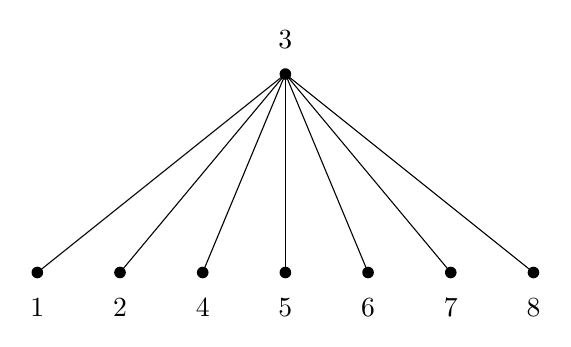
\begin{tikzpicture}[baseline=(current bounding box.center), scale=1.05]
  \coordinate (vc3) at (0,2.4);
  \fill (vc3) circle (2pt);
  \node[inner sep=1pt] at (0,2.82) {3};
  \foreach \x/\lab in {-3/1,-2/2,-1/4,0/5,1/6,2/7,3/8} {
    \coordinate (vc\lab) at (\x,0);
    \fill (vc\lab) circle (2pt);
    \node[inner sep=1pt] at (\x,-0.42) {\lab};
    \draw (vc3) -- (vc\lab);
  }
\end{tikzpicture}
&
$V = \{\cancel{1}, \cancel2, \underline{3}, \cancel{4}, \cancel{5}, \cancel{6}, \cancel{7}, \underline{8}\}$
\end{tabular}
\end{center}
\noindent\textbf{\underline{3.2}}\par
\vspace{0.75\baselineskip}
\noindent
\textbf{4.} \begin{tabular}[t]{l}
    Test the graph whose adjacency matrix is given below to see if it is connected.
\end{tabular}\par
\vspace{0.75\baselineskip}
\begin{center}
\renewcommand{\arraystretch}{1.25}
$\begin{array}{c|cccccccc}
    & x_1 & x_2 & x_3 & x_4 & x_5 & x_6 & x_7 & x_8 \\ \hline
x_1 & 0 & 0 & 1 & 0 & 0 & 1 & 0 & 1 \\
x_2 & 0 & 0 & 1 & 0 & 1 & 0 & 1 & 0 \\
x_3 & 1 & 1 & 0 & 1 & 0 & 0 & 0 & 0 \\
x_4 & 0 & 0 & 1 & 0 & 1 & 1 & 1 & 0 \\
x_5 & 0 & 1 & 0 & 1 & 0 & 0 & 0 & 1 \\
x_6 & 1 & 0 & 0 & 1 & 0 & 0 & 0 & 0 \\
x_7 & 0 & 1 & 0 & 1 & 0 & 0 & 0 & 1 \\
x_8 & 1 & 0 & 0 & 0 & 1 & 0 & 1 & 0
\end{array}$
\end{center}
\begin{center}
    * To see if a graph is connected, apply BFS
\end{center}
\vspace{0.75\baselineskip}
\begin{center}
\begin{tabular}{c@{\hspace{1.25em}}c}
$\Rightarrow$ &
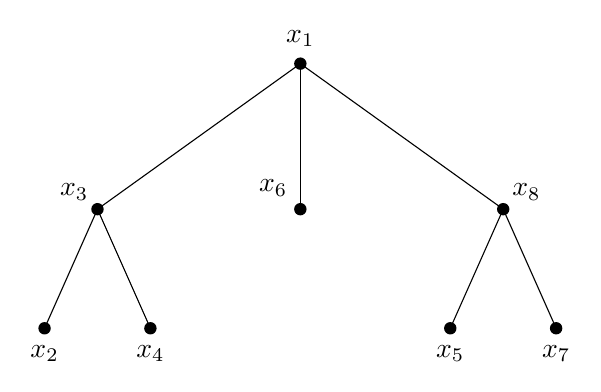
\begin{tikzpicture}[baseline=(current bounding box.center), scale=1.12]
  \coordinate (x1) at (0,3);
  \coordinate (x3) at (-2.3,1.35);
  \coordinate (x6) at (0,1.35);
  \coordinate (x8) at (2.3,1.35);
  \coordinate (x2) at (-2.9,0);
  \coordinate (x4) at (-1.7,0);
  \coordinate (x5) at (1.7,0);
  \coordinate (x7) at (2.9,0);
  \draw (x1) -- (x3);
  \draw (x1) -- (x6);
  \draw (x1) -- (x8);
  \draw (x3) -- (x2);
  \draw (x3) -- (x4);
  \draw (x8) -- (x5);
  \draw (x8) -- (x7);
  \foreach \p in {x1,x2,x3,x4,x5,x6,x7,x8} {\fill (\p) circle (2pt);}
  \node[above=5pt, inner sep=1pt] at (x1) {$x_1$};
  \node[above left=3pt, inner sep=1pt] at (x3) {$x_3$};
  \node[above left=5pt, inner sep=1pt] at (x6) {$x_6$};
  \node[above right=3pt, inner sep=1pt] at (x8) {$x_8$};
  \node[below=5pt, inner sep=1pt] at (x2) {$x_2$};
  \node[below=5pt, inner sep=1pt] at (x4) {$x_4$};
  \node[below=5pt, inner sep=1pt] at (x5) {$x_5$};
  \node[below=5pt, inner sep=1pt] at (x7) {$x_7$};
\end{tikzpicture}
\end{tabular} 
\end{center} 
\begin{center}
    \boxed{\text{Since every vertex is visited, this graph is connected.}}
\end{center}
\end{document}